\documentclass[12pt]{article}                   % Začátek dokumentu
\usepackage{../../MFFStyle}                     % Import stylu

\begin{document}
	Budeme chtít najít kořeny funkce $f(x) = x^2 - x - 2$ pomocí metod pevného bodu.
	$$ \phi_1(x) = x^2 - 2, \qquad \phi_2(x) = \sqrt{x + 2}, \qquad \phi_3(x) = 1 + \frac{2}{x}, \qquad \phi_4(x) = \frac{x^2 + 2}{2x - 1}. $$

\begin{priklad}[4.1]
	Popište, jak jsou jednotlivé metody $\phi_1, …, \phi_4$ odvozeny.

	\begin{reseni}
		$$\begin{array}{c c c c c}
			x = \phi_1(x) = x^2 &\overset{/-x}{\Leftrightarrow}& 0 = x^2 - x - 2 = f(x), && \\
			x = \phi_2(x) = \sqrt{x + 2} &\overset{/·^2}{\implies}& x^2 = x + 2 &\overset{/-x-2}{\Leftrightarrow}& f(x) = x^2 - x - 2 = 0, \\
			x = \phi_3(x) = 1 + \frac{2}{x} &\overset{/·x}{\implies}& x^2 = x + 2 &\overset{/-x-2}{\Leftrightarrow}& f(x) = x^2 - x - 2 = 0, \\
			x = \phi_4(x) = \frac{x^2 + 2}{2x - 1} &\overset{/·(2x - 1)}{\implies}& 2x^2 - x = x^2 + 2 &\overset{/-x^2-2}{\Leftrightarrow}& f(x) = x^2 - x - 2 = 0. \\
		\end{array}$$
	\end{reseni}
\end{priklad}

\begin{priklad}[4.2]
	Platí pro všechny metody $\phi_1, …, \phi_4$, že jsou oba kořeny $f$ pevnými body?

	\begin{reseni}
		Platí to pro $\phi_1$, protože děláme ekvivalentní úpravu a pro $\phi_3$ a $\phi_4$, protože tam jsou pro úpravu problémové body $0$ a $\frac{1}{2}$. Pro $\phi_2$ to neplatí, protože úprava není ekvivalencí pro záporná $x$, tedy ani pro $-1$. Můžeme vidět, že $\phi_2(-1) = 1$.
	\end{reseni}
\end{priklad}

\begin{veta}
	Nechť $\phi(\overline x) = \overline x$ a nechť $I, \overline x \in I$, je interval takový, že platí:
	\begin{itemize}
		\item $\phi \in ©C^1(I)$,
		\item $|\phi'(x)| < 1$ $\forall x \in I$,
		\item $\phi(I) \subseteq I$.
	\end{itemize}
	Pokud $x_0 \in I$, pak iterace pevného bodu konverguje do $\overline x$.
\end{veta}

\pagebreak

\begin{priklad}[4.3]
	Je možné pomocí předchozí věty ukázat, zda budou jednotlivé metody konvergovat pro danou volbu počátečního bodu? Pokud ano, ukažte. $x_{0, \phi_1} = 3$, $x_{0, \phi_2} = -1.5$, $x_{0, \phi_3} = 3$, $x_{0, \phi_4} = 0$.

	\begin{reseni}
		Pro $\phi_1$ nelze větu použít, jelikož $x_0 = 3 \in I$ a $\phi'(x_0) = 2x_0 = 6 > 1$. (Navíc $\phi_1$ pro $x_0 = 3$ nekonverguje, ale diverguje k $+∞$, protože $x^2 - 2 > 2x$ pro všechna $x ≥ 3$, tj. diverguje rychleji než $2^n$.)

		Pro $\phi_2$ zvolíme $I = \[-1.5, +∞\)$, $\phi_2'(x) = \frac{1}{2}\frac{1}{\sqrt{x + 2}}$ je zřejmě spojitá pro $x > -2$, tedy na celém $I$, zároveň pro $\sqrt{x + 2} > 0.5$, tj. pro $x > -1.75$ (tj. na celém $I$), je $0 < \phi_2'(x) < 1$. $\phi_2$ zobrazuje do kladných čísel, tedy do $I$ (a je na celém intervalu $I$ definováno), takže platí i třetí bod. Pevným bodem je $2 \in I$ (a $x_0 = -1.5 \in I$), tedy tato metoda konverguje.

		Pro $\phi_3$ zvolíme například interval $\(\sqrt{2}, 3\] = I$, kde $0 > \phi_3'(x) = -\frac{2}{x^2} > -1$ je spojitá a $x_0 = 3 \in I$ a $\overline x = 2 \in I$. Jediné, co zbývá ověřit je $\phi_3(I) \subset I$, ale $\phi_3$ je klesající a $\phi_3(3) = 1.5 > \sqrt{2}$ a $\phi_3(\sqrt{2}) = 1 + \sqrt{2} < 3$. Tedy také tato metoda konverguje podle věty výše.

		Pro $\phi_4$ a $x_0 = 0$ nelze větu použít přímo, protože $x_0 \in I$ a $\phi_4'(x_0) = 2\frac{x_0^2 - x_0 - 2}{(2x_0 - 1)^2} = -4 < -1$, ale můžeme si všimnout (např. z následující úlohy), že pro $\tilde x_0 = \phi_4(x_0) = \frac{0^2 + 2}{2·0 - 1} = -2$ už můžeme zvolit interval $[-2, -1] = I$, kde $0 ≤ \phi_4'(x) = 2\frac{x^2 - x - 2}{(2x - 1)^2} < \frac{1}{2} < 1$ je spojitá. Zároveň $\tilde x_0, \overline x = -1 \in I$ a $\phi_4(I) = \[-\frac{6}{5}, -1\] \subseteq I$. Tedy $\phi_4$ pro $x_0 = 0$ konverguje podle předchozí věty a toho, že $\phi_4(x_0) = -2 = \tilde x_0$.
	\end{reseni}
\end{priklad}

\begin{priklad}
	Chování metody pevných bodů z předchozí úlohy otestujte pomocí náčrtu. Pokud metoda konverguje, přestože věta nešla použít, zdůvodněte proč.

	\begin{reseni}
		$\phi_1$ prostě nekonverguje, $\phi_2$ a $\phi_3$ konvergují podle\\
		věty a $\phi_4$ už jsem vysvětlil v předchozí úloze.\\[-4em]
		
		\noindent\raise 0.2em\hbox{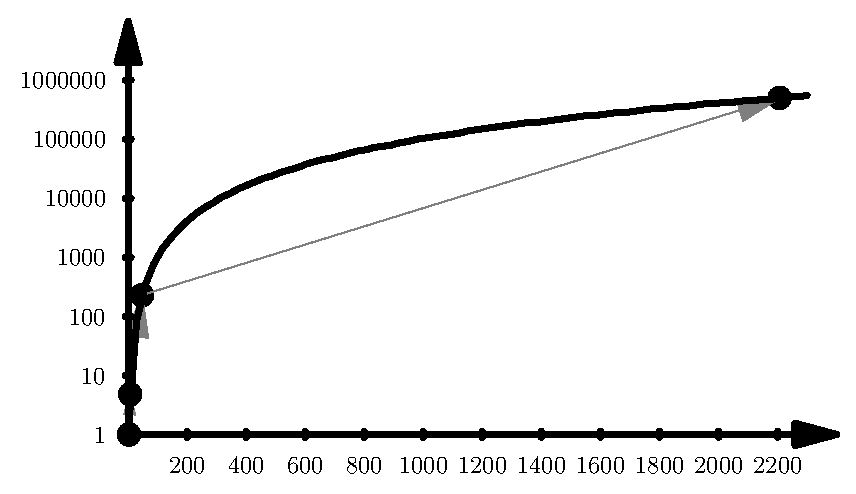
\includegraphics[width=0.3\textwidth]{NDU4_phi1.eps}}
		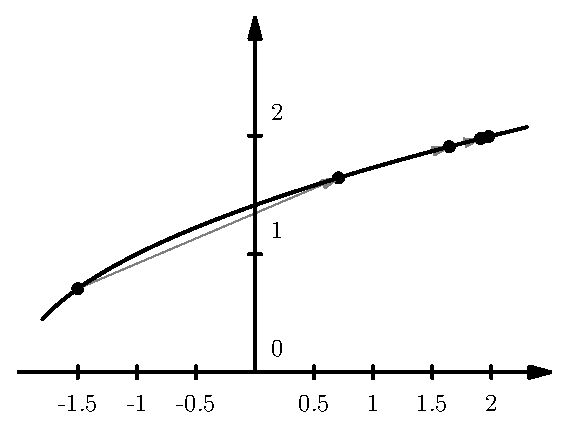
\includegraphics[width=0.25\textwidth]{NDU4_phi2.eps}
		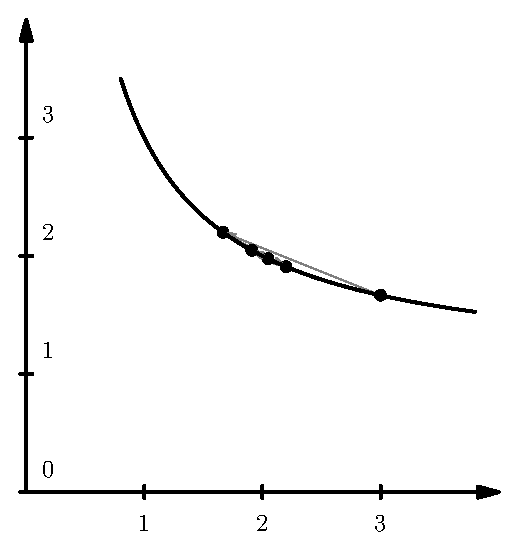
\includegraphics[width=0.25\textwidth]{NDU4_phi3.eps}\hspace{-2em}
		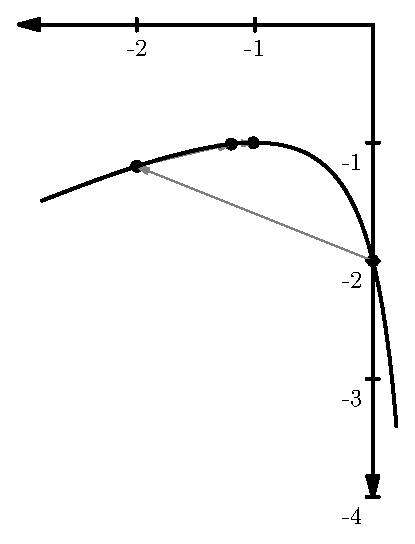
\includegraphics[width=0.2\textwidth]{NDU4_phi4.eps}\\[-2em]

		\noindent\hspace{0.15\textwidth}$\phi_1$\hspace{0.23\textwidth}$\phi_2$\hspace{0.25\textwidth}$\phi_3$\hspace{0.23\textwidth}$\phi_4$
	\end{reseni}
\end{priklad}

\end{document}
